\section{Memory Access Optimization}
\label{sec:access}
% after trafer of memory
After memory transfer, it is important to access the transfered data efficiently.\\
Both access to global and shared memory obey access constraints and to fully optimize CUDA applications it is important
to follow several requirements which we will examine below.
\subsection{Global Memory Access}
%\cite{pfa_access_global}
\label{global_access}
% only mem av from host
Global memory is arguably the most important memory in a GPU with the vast amount of memory available and its global scope.\\
Though the bandwidth is very high with well over 100 GB/s on current hardware, it may be decreased heavily by uncoalesced access patterns which we will dissect now.\\
\subsubsection{Theoretical Bandwidth}
%\cite{http://devblogs.nvidia.com/parallelforall/how-implement-performance-metrics-cuda-cc/}
In evaluating and optimizating global memory access and its throughput it is useful to have a metric to compare against.\\
This can be provided by the theoretical bandwidth peak which allows approximation of device memory bandwidth capabilities. It has to be emphasized that this is only the theoretical possible bandwidth, which shows if more optimization is needed as the first optimizations can generally be quite simple.\\
$$ BW_{\mathrm{theoretical}} = CLK \times \mathrm{Width}_{\mathrm{Bus}} \times DDR $$
Where $CLK$ is the clock rate (which can vary depending on GPU boost) and $\mathrm{Width}_{\mathrm{Bus}}$ is the memory bus width and $DDR$ can be two due to double data rate used by modern GPU.\\
% todo citation
Using this formula, the theoretical bandwidth for a system with a GDDR5 memory clocked at 1.8 GHz and a 384-bit wide bus results in \SI[per-mode=symbol]{168}{\gibi\byte\per\second}.
% todo citation
%\cite{cuda_handbook_5.2.13_ecc}
The achieved bandwidth can also be lowered by error correcting code (ECC), which can correct 1-bit and report 2-bit memory errors by about $20\%$. 
\subsubsection{Coalesced Access}
As mentioned in \ref{hardware_global}, CUDA tries to merge memory requests from a warp together in order to improve global memory performance.\\
While CUDA GPUs with better hardware capabilities have emerged, the hardware and algorithms to merge memory requests have also improved,
however CUDA applications striving for high performance will still have to optimize its memory access.\\
There are several factors to pay attention to when addressing accessing global memory:\\
\begin{itemize}
    \item Only access to 1, 2, 4, 8 and 16 bytes of global memory will compile to a single instruction.
    \item Accessed data has to be naturally aligned, i.e. its address has to be a multiple of its size.
    \item Access patterns following the hardware guidelines have to be used.
    \item more-dimensional data have to aligned correctly to provide coalesced access, see \ref{2d_access} for details.
\end{itemize}

%\subsubsection{memory requests / memory transactions}
%\subsubsection{size and alignment}
% misalignment doesnt matter in cc 2.x up
\subsubsection{Aligning Structures}
Like all other global memory access, structures have to be aligned to have its access coalesced.\\
It is possible to enforce this behaviour using the compiler keyword  $\_\_align(n)\_\_$
where now the structure have its starting address aligned to a multiple of $n$.\\
Additionally, if the size of the structure is not a multiple of $n$, an array of the structure will be padded to have its size aligned as well.\\
For example the structure $testStruct$ (name...) is now aligned to at least 32 bytes:\\
\begin{lstlisting}[language=c]
struct __align__(8) testStruct {
    uint16_t a, b, c;
}
\end{lstlisting}

% todo: test!!!
% 
Normally, without the $\_\_align\_\_$ keyword, this structure would have a size of 6 bytes but to have its
size aligned to a multiple of 8, it is padded using another 2-byte word.\\

\subsubsection{Strided Memory Access}
While misaligned accesses on more current hardware have lower impact on performance than before\cite{pfa_access_global}, due to more advanced coalescing techniques and hardware,
strided access is still a problem and will continue to be challenging.\\
This comes at no surprise, because when threads in warp access memory at locations far apart, there is no way for the hardware to merge its memory requests and provide coalesced access.\\
\begin{figure}[H]
    \centering
    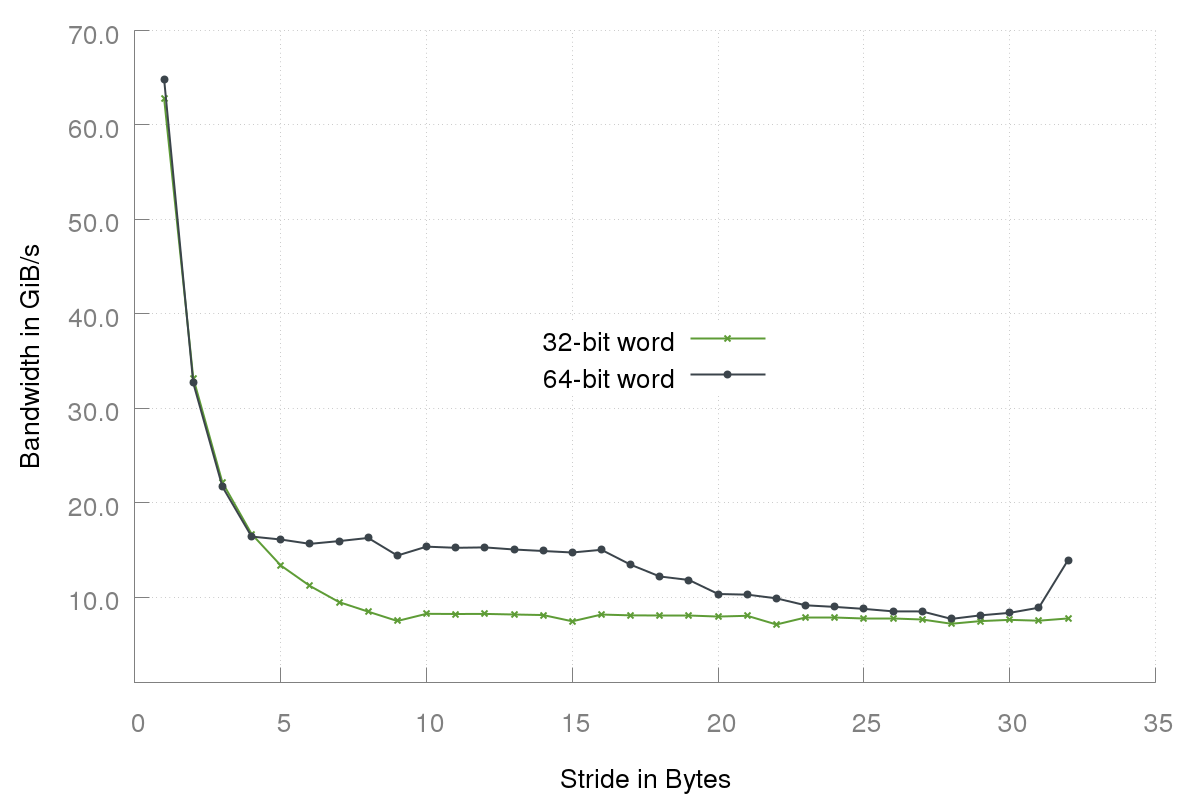
\includegraphics[scale=0.18,natwidth=1200,natheight=800]{media/strided_bandwidth.png}
    \caption{Strided Access on current hardware\\\hspace{\textwidth}hi test test2}
    \caption*{Test system: NVIDIA GTX 750 1GB CC 5.0, CUDA 7.5}
    \caption*{Source code: \href{https://github.com/spotlight0xff/cuda\_paper/code/coalescing\-global/}{On GitHub}\cite{pfa}}
    \label{fig:strided_access}
\end{figure}
Figure~\ref{fig:strided_access} illustrates the memory throughput using the following strided memory access pattern on 32-bit and 64-bit word sizes.\\
$$ (blockDim.x \times blockIdx.x + threadIdx.x) \times \mathrm{stride} $$
%Surprisingly, 
As expected, strided access proves to be impactful on the performance although surprisingly,
64-bit data has a higher throughput compared to 32-bit.\\
% TODO explanation or fuck off
This can be mitigated by using shared memory to manually cache the strided data in shared memory in a coalesced fashion. As we will see later, shared memory does not punish for strided access.\\
\subsubsection{Latency Hiding through Thread Parallelism}
Even though some kernels may be latency-bound,
that is when the kernel execution depends on the latency of global memory to continue execution,
this may not effect the performance using high enough block size.\\
%todo clarify
Because of how the SM schedules warps for execution,
if enough warps are waiting to be executed, some warps waiting to complete a memory request can be skipped.\\
This is only because of how lightweight threads are implemented on GPU in comparison to traditional threads on a CPU where each time a context switch is performed, registers have to be restored.
Contrary to that, on a GPU a context switch does \emph{not} perform any expensive operation as the registers are all stored on the multiprocessor and can be used directly.\\
Quoting a NVIDIA presentation, to hide math and memory latency about``~512 threads per SM'' \cite{sc11_perf_optimization} are needed.\\
%As said, each microarchitecture has different constrains, which we will discuss below.
\subsubsection{Fermi-class hardware (CC 2.x)}
%\cite{cuda_handbook_global_memory_sm2_x}
Devices of compute capability 2.x will cache global memory accesses by default in both L1 and L2 cache,
though this behaviour can be changed to cache only in L2 with a compiler switch.\\
While requests served by both L1 and L2 cache will result in 128-byte transactions, requests only operating on L2 cache result in 32-byte transactions.\\
Therefore it is sometimes useful to use only L2 cache, as in the case of scattered or random access to avoid fetching too much data.\\

%Contrary to devices of compute capability 1.x, Ferm-class hardware will coalesce access to global memory within a whole warp
%and cache by default in L1 and L2 cache, though this can be changed to caching only in L2 with a compiler switch.\\
%Caching only in L2 may be useful to reduce overfetch for scattered or random access, as L2 cache lines are only 32-byte (cache segments??)
%while L1 cache contains 128-byte cache lines and reduce therefore overfetch.

%On Fermi-class hardware is global memory access by default cached in both L1 and L2 cache.

%Beginning with Fermi, the L1 cache with lines of 128 byte are used to cache access to global memory.\\

%Global memory will be served using both caches ( though this can be changed using compiler directives, using \emph{-Xptcas -dlcm=cg} to just L2 cache), 
\subsubsection{Kepler-class hardware ( SM 3.x)}

With Kepler all global memory access is cached through L1 while L2 is reserved for local memory requests.\\
Starting with SM 3.5, chips have the capability to use the texture cache to fulfil memory requests as well.\\
\subsubsection{Maxwell-class hardware (SM 5.x)}

\subsubsection{Two Dimensional Access}
%\cite{shane_global_memory}
%\cite{http://docs.nvidia.com/cuda/cuda-c-programming-guide/index.html#device-memory-accesses}
\label{2d_access}
To use coalescing access to two-dimensional data
\footnote{I will focus on two-dimensional arrays only, but the same theory applies to data in more dimensions},
it is needed to have a correctly aligned array.
For instance if an array of 50 rows with each 30 float values is needed,
a call to cudaMalloc with the requested size of $ 50 \times 20 \times sizeof(float) $ results in a allocated memory of 4000 bytes.
The problem occurs when accessing the first element of the second row, i.e. $ values[1][0] $.
The address of this element equals the length of a row which is 50 bytes. This is not a multiple of the warp size, which may result in uncoalesced access.\\
Therefore it is desired to have arrays with dimensions according to coalescing constrains.
For convenience CUDA provides the possibility to allocate so-called \emph{pitched memory},
that is mostly more-dimensional memory with a padding aligned to meet the hardware requirements for coalesced access.\\
To use this feature, \emph{cudaMallocPitch()} and \emph{cudaMalloc3D()} are available for two-dimensional and three-dimensional arrays, respectively.\\
Indexing a pitched 2D memory works with the following formula:\\
$$ (base + row * pitch) + column$$\\
This technique allows on all hardware fully coalesced access and also transfer using \emph{cudaMemcpy2D()} and \emph{cudaMemcpy3D()}.\\
\subsection{Shared Memory Access}
\label{shared_access}
Due to being on-chip, shared memory has extremly fast access times and very high bandwidth for threads on the multiprocessor. Therefore it is mostly used to exchange and synchronize between threads in a block.\\
Shared memory is accessed using 32 memory banks, which are able to maintain a bandwidth of 32 bits every clock cycle and every two clock cycles for Fermi and Maxwell devices, respectively.\\
Kepler devices are able to switch between word sizes of 32-and 64-bit width to enable fast shared memory access to 64-bit values like $doubles$, though this mode has been dropped due to increased simplicity in Maxwell devices.\\
% todo: why dropped? + cite
This memory bank concept enables high performance concurrent access where the resulting bandwidth is 32 times higher than the bandwidth of a single memory bank given that no bank conflicts occur.\\
Memory banks are organized in a way that successive word are assigned to successive memory banks.\\
When $n$ threads with $n>1$ try to access the same bank requesting a different word, the access is serialized and the bandwidth is lowered and a $n$-way bank conflict occurs.\\
If the same word within a memory bank is accessed by all threads or multiple threads in a warp no bank conflict is generated as the value is respectively broadcasted or multicasted to the requesting threads.\\
